\chapter{相关技术及原理}
本章对研究工作相关基础理论和技术原理做详细介绍,
主要包括数据增强技术、深度卷积神经网络及其核心原理、
模型参数训练涉及的损失函数和最优化方法等。

%————————————————————————————————————————————2.1 数据预处理——————————————————————————————————————————————————————————————————————————
\section{数据预处理}
深度学习模型十分依赖大数量、高质量的数据集,数据集的数量和质量对于训练模型参数、促进模型拟合、提高模型预测和泛化能力十分重要。
因此,针对现有数据集进行相应的数据预处理,是解决数据噪声多、数据量少、数据多样性不足、数据分布不均衡等问题的重要前置手段。
道路裂缝图像的数据预处理方法,包括图像去噪、图像增广、图像增强、数据变换等。
\subsection{图像去噪}
路面裂缝图像是基于摄像机,采集自真实的道路路面,受光照、灰尘、水渍等自然因素和摄像器件老化、电流噪声、电磁干扰等物理因素影响较大,导致图像在采集和传输过程中引入异常值和噪声。
图像去噪主要针对裂缝图像中的异常值和噪声进行相应的去噪和剔除,常见的图像去噪方法包括均值滤波、中值滤波和卡尔曼滤波等。

\textbf{(1)均值滤波}

均值滤波基于滑动窗口,对邻域内的像素取平均值,作为当前像素点的值,是一种常见的图像平滑滤波方法。公式如下:
\begin{equation}
	\bm{I^{~'}}(x, y) = \frac{1}{k^2}\sum_{(i, j)\in A_k}\bm{I}(x_i, y_j)
\end{equation}
上述公式中,A表示k*k的滑动窗口,$I^{~'}(x, y)$表示取均值后的像素值。均值滤波是一种线性的滤波算法,对图像中的异常值比较敏感,容易受特殊异常值影响。均值滤波的效果图,如下图所示:

\begin{figure}[H]
	\subfloat[]{
		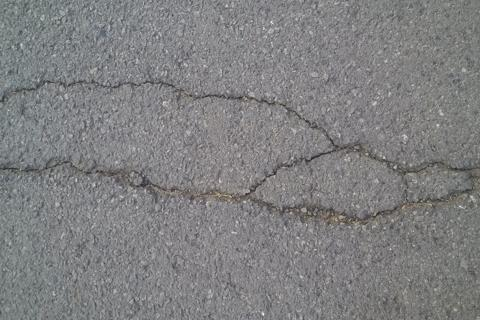
\includegraphics[width=6cm, height=4cm]{pic/input-filter.png}
	}
	\subfloat[]{
		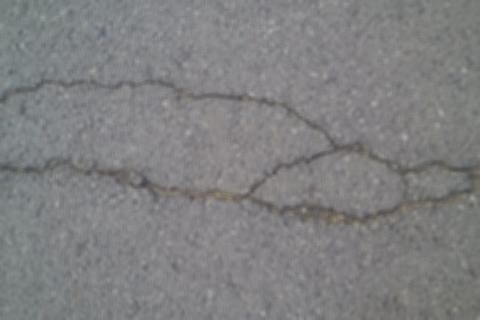
\includegraphics[width=6cm, height=4cm]{pic/mean_filtered.png}
	}
	\caption{图像均值滤波效果图}
	\label{mean}
\end{figure}

\textbf{(2)中值滤波}

中值滤波是一种非线性的平滑滤波方法,其对领域内的像素取中值,作为当前像素点的值,该滤波方法相比平均滤波,适合去除椒盐噪声。公式如下:
\begin{equation}
	\bm{I^{~'}}(x, y) = \bm{median}_{(i, j)\in A_k}\bm{I}(x_i, y_j)
\end{equation}
其中,A表示k*k的滑动滤波窗口,$I^{~'}(x, y)$取中值后的像素值。中值滤波的效果图,如下图所示:

\begin{figure}[H]
	\subfloat[]{
		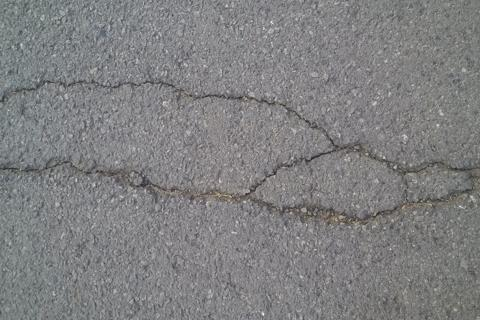
\includegraphics[width=6cm, height=4cm]{pic/input-filter.png}
	}
	\subfloat[]{
		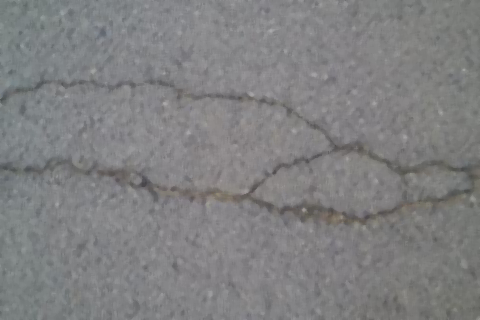
\includegraphics[width=6cm, height=4cm]{pic/median_filtered.png}
	}
	\caption{图像中值滤波效果图}
	\label{median}
\end{figure}

\textbf{(3)高斯滤波}

高斯滤波是一种利用高斯函数对像素点进行卷积,即基于权重取平均的方法。该算法也是对邻近像素点赋予更高权重,对远处像素点赋予更低的权重,是对均值滤波的一种改善和优化。公式如下:
\begin{equation}
	\bm{I^{~'}}(x, y)= \sum_{(i, j)\in A_k}\bm{G}(i, j)\bm{I}(x_i, y_j)
\end{equation}
其中,A依然表示k*k的滑动滤波窗口,$I^{~'}(x, y)$取中值后的像素值,
高斯函数$G(i, j) = \frac{1}{2\pi\sigma^2}e^{-\frac{i^2+j^2}{2\sigma^2}}$表示领域像素点的权重,高斯滤波的效果,如下图所示:

\begin{figure}[H]
	\subfloat[]{
		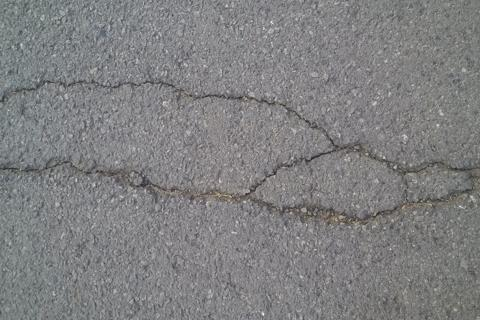
\includegraphics[width=6cm, height=4cm]{pic/input-filter.png}
	}
	\subfloat[]{
		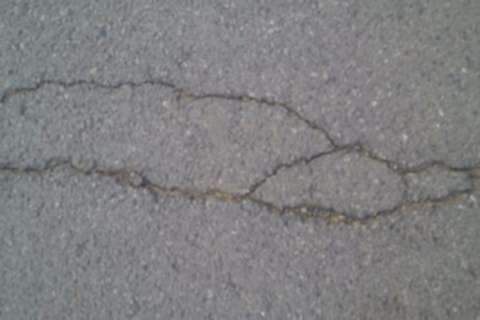
\includegraphics[width=6cm, height=4cm]{pic/gaussian_filtered.png}
	}
	\caption{图像高斯滤波效果图}
	\label{gaussian}
\end{figure}

均值滤波能一定程度上平滑图像,但是对异常值比较敏感,容易受到特殊异常值影响,比如重尾的椒盐噪声;高斯滤波在一定程度上减轻了对椒盐噪声的敏感程度,而且能较好地保留局部特征;然而,均值和高斯滤波两者都容易模糊边缘,造成
边缘信息丢失。中值滤波,是一种非线性地滤波方法,不仅能有效去除椒盐噪声,而且对高斯噪声有一定效果,还能较好地保留边缘。
根据上述实验结果,对于裂缝图像这种边缘信号比较重要的检测场景,中值滤波是一种更适合的去噪算法。

考虑到提高模型的抗干扰能力,适当的图像噪声反而有利于增强模型的泛化能力和鲁棒性。因此,图像去噪在模型参数训练阶段可以选择不做,其适合放在模型部署和推理的数据预处理阶段进行,能有效提高模型推理的精度。

\subsection{图像增广}
实际场景下,道路裂缝图像采集工作耗时费力,想要采集大量的道路裂缝图像难度较大。因此,对现有数据集进行数据增广,以增加裂缝图像数量和多样性,是数据预处理阶段的重要工作之一。
图像增广(Image Augmentation)是对原始图像进行翻转、缩放、剪切、色彩变换等操作,从而增加图像数量和多样性、提高模型泛化能力和鲁棒性的方法。
常见的图像增广方法,主要包括仿射变换、色彩变换等。

\textbf{(1)仿射变换}

仿射变换,也叫几何变换,指的是对原始图像进行上下左右翻转、旋转、平移、缩放、剪切及其组合的操作。
仿射变换是一种受仿生学启发的数据增广方法,其模拟生物组织的形变特性,利用翻转、缩放等手段,对图像进行
弹性变形,从而从几何上增加图像的多样性,在深度学习数据增广领域应用广泛。公式如下:
\begin{equation}
	\begin{bmatrix}
		x \\
		y \\
		1
	\end{bmatrix}
	=
	\bm M
	\begin{bmatrix}
		x_0 \\
		y_o \\
		1
	\end{bmatrix}
\end{equation}
其中,$(x_0\ y_0\ 1)^T$是像素点的原位置坐标,$(x\ y\ 1)^T$是变换后的位置坐标,M是一个$3\times3$的仿射变换矩阵,该矩阵表示翻转、旋转、缩放等变换信息。

当$M=\begin{bmatrix}
	-1 & 0 & W \\
	 0 & 1 & 0 \\
	 0 & 0 & 1 
\end{bmatrix}$
时,W为图像宽度,原公式表示水平翻转。
图像水平翻转效果,见下图\ref{horizon-test}所示。

\begin{figure}[H]
	\subfloat[]{
		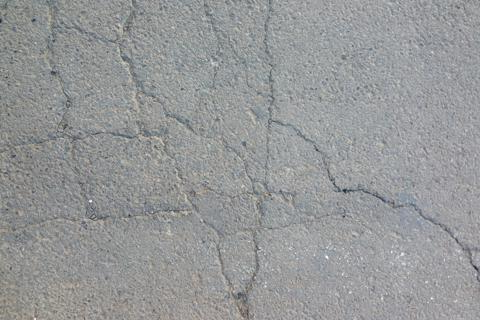
\includegraphics[width=6cm, height=4cm]{pic/horizon-test-pre.png}
		\label{horizon-test-pre}
	}
	\subfloat[]{
		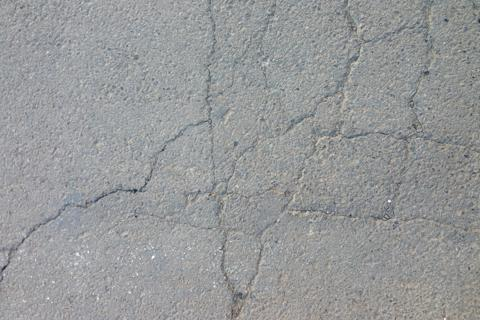
\includegraphics[width=6cm, height=4cm]{pic/horizon-test-post.png}
		\label{horizon-test-post}
	}
	\caption{图像水平翻转效果图}
	\label{horizon-test}
\end{figure}

当$M=\begin{bmatrix}
     S_x & 0 & W \\
	 0 & S_y & 0 \\
	 0 & 0 & 1 
\end{bmatrix}$
时,$S_x$、$S_y$为宽、高缩放比例,原公式表示图像缩放。

\textbf{(2)色彩变换}

色彩变换,区别于仿射几何变换,色彩变换不是对像素位置坐标的变换,而是对像素信号值本身的调整和变换,包括图像亮度、对比度等调整。
受限于光照、灰尘等自然因素和感光元件、电磁干扰等物理因素影响,对原始图像进行色彩变换,可以进一步增加图像在
色彩空间上的多样性,更好地模拟各种干扰情形。
其中,亮度变换是对像素点灰度值或者RGB色彩空间值,按照一定比例增大或者缩小,实现图像亮度变亮或者变暗。
对比度变换则是增大或减小像素点的亮度值差异。业界常见的亮度、对比度调节算法包括形态学方法和直方图均衡化方法。本文基于相关算法,进行图像色彩空间变换。
其中,亮度减小和对比度增加的效果,见下图\ref{contrast-test}所示

\begin{figure}[H]
	\subfloat[]{
		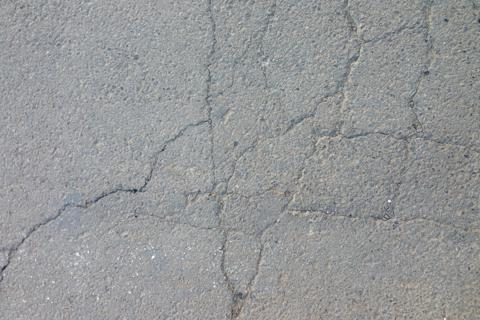
\includegraphics[width=6cm, height=4cm]{pic/contrast-test-pre.png}
		\label{contrast-test-pre}
	}
	\subfloat[]{
		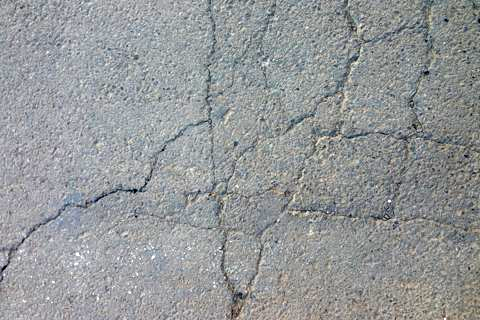
\includegraphics[width=6cm, height=4cm]{pic/contrast-test-post.png}
		\label{contrast-test-post}
	}
	\caption{图像对比度增加效果图}
	\label{contrast-test}
\end{figure}

本文的裂缝图像,主要基于仿射变换、色彩变换进行数据增强,不仅能够增加数据集的数量,而且能够增加数据的多样性,充分
考虑各类自然光照、灰尘、亮度、对比度、位置、角度、形状等不同变量和影响因素,促进模型训练参数拟合,进一步提高裂缝检测
模型的鲁棒性和泛化能力。

\subsection{图像归一化}
基于灰度或者RGB色彩空间的图像,其像素值往往较大。图像像素归一化,是计算机视觉领域的标准操作之一,
其目的是将像素归一化到$[0,1]$之间,有利于加速模型收敛和优化。公式如下:

\begin{equation}
	I_c = \frac{I_0-I_{min}}{I_{max}-I_{min}},\ c\in {\{Red,Green,Blue,Gray\}}
\end{equation}
其中,$c$表示相应色彩通道,$I_0$原像素值,$I$表示标准化后的像素值。

%————————————————————————————————————————————2.2 深度卷积神经网络——————————————————————————————————————————————————————————————————————————
\section{深度卷积神经网络}
卷积神经网络(Convolutional Neural Net,CNN)最初由Lecun Yang等\citing{cnn}在1989年提出。
这篇论文展示了卷积神经网络LeNet在手写数字识别数据集上的应用,并详细介绍了有关CNN的卷积层、池化层(当时被称为子采样层)和
全连接层,以及基于反向传播算法进行模型的参数训练。

\subsection{CNN提出的意义}
在CNN之前,传统的多层感知机(Multilayer Perceptron,MLP)在处理数据时,其隐藏层每一个输入神经元节点会与每一个输出神经元节点相连接,构成全连接层(Fully Connected Layer,FC)。
这种层结构能够实现全局特征提取,避免特征信息的丢失,在处理文本等序列数据时十分重要。然而,全连接层在处理图像等二维空间结构更复杂的数据时,会导致层参数量暴增,大大增加了模型训练的难度。
例如,一个$1000\times1000$分辨率的图像,假设采用RGB三通道表示,即使隐藏层数降低到1000层,模型也会达到$1000^2\times3\times10^3=3\times10^9$个参数。如此庞大的数据量对于GPU等硬件是难以承受的,
训练效率会大大降低。

然而,图像等二维空间结构数据,相比文本等序列数据,具有位移不变性和空间局部性两个新的数据特性。下面对这两个特性做出详细介绍,并基于此改进传统全连接的层结构。

\textbf{(1)位移不变性}

假设计算机要识别找出一个图像中的猫,那么基于常理可知,猫的位置不会影响识别效果。即使猫从A位置移动到了B位置,计算机对猫的识别和反应应该在不同位置是相似或者一样的,不应随位置空间而改变。这就是
图像这种空间数据,区别于文本等序列结构数据的关键,图像数据并不对位置和序列产生要求。
基于图像数据的位移不变性,可以做出以下推导:

假设对一个$w\times{h}$的灰度单通道图像$X$进行分类,其中,$w$表示图像的宽度,$h$表示图像的高度。
$X(x\in{(i,j)})$作为输入层神经元节点,$X_{i,j}$表示原图像在输入层节点$(i,j)$的像素值。
$H_{q,v}$表示隐藏层节点$(q,v)$的输出值。
${W}_{q,v,i,j}$表示隐藏层节点$(q,v)$在输入层节点$(i,j)$上权重参数,$W$是一个四维的权重张量。
$B_{q,v}$表示隐藏层节点$(q,v)$的偏置参数。

全连接层的形式化表达如下:
\begin{equation}
	\bm{H}_{q,v} = \sum_{i}^{w}\sum_{j}^{h}\bm{X}_{i,j}\bm{W}_{q,v,i,j} + B_{q,v}
\end{equation}
根据上式,假设隐藏层的数量为$n$,由于此处隐藏层采取全连接方式,其参数量为$n\times{w}\times{h}$个,参数量较大。

基于图像数据的位移不变性,上述公式可以修改为:
\begin{equation}
	\bm{H}_{q,v} = \sum_{i}^{w}\sum_{j}^{h}\bm{X}_{i,j}\bm{W}_{i,j} + B
	\label{parameter_sharing}
\end{equation}
该式中,所有隐藏层共享同一权重参数和偏置参数,此时隐藏层的参数量为$w\times{h}$个参数,相比全连接的隐藏层参数量少了一个数量级,
参数量的大幅减小,十分有利于模型参数训练。

\textbf{(2)空间局部性}

在图像数据中,邻域内所表达信息的是相似的,并且神经网络在对图像做分类或者分割时,前期的隐藏层应当专注于探索图像
的局部特征,而非全局特征和长距离依赖关系。比如,在目标检测中,用户关注的是目标是否存在和目标所在的位置坐标,此时图像局部特征的提取对于目标检测和定位更为重要,而非全局信息;
图像分类中,在网络输出时,基于全连接层提取全局特征,输出各个类别的概率,而前期隐藏层只需关注局部特征即可。
此时,公式\ref{parameter_sharing}可以修改为:
\begin{equation}
	\bm{H}_{q,v} = \sum_{i=i-\Delta}^{i+\Delta}\sum_{j=j-\Delta}^{j+\Delta}\bm{X}_{i,j}\bm{W}_{i,j} + B
\end{equation}
其中,$\Delta$表示选取输入层节点$(i,j)$周围边长为$\Delta$的邻域,此时,隐藏层节点将局部输入层节点作为输入,从而实现对图像局部信息的提取,其参数量将会进一步减少为$(2\times{\Delta})^2$个。
因此,选取部分相邻的输入层节点输入到隐藏层,不仅可以有效提取图像的局部特征,方便图像处理,而且可以在参数共享的基础上,进一步大幅减小模型的参数量。

综上所述,要解决传统多层感知机在图像数据处理上的限制,必须基于图像数据的位移不变性和空间局部性两大特征,
实现参数共享和局部特征提取,从而大幅减少模型隐藏层的参数量,
这样的隐藏层,就是卷积神经网络CNN中的提出的卷积核(Convolution Kernal),亦称作滤波器(Filter)。

\subsection{卷积层}
卷积层是卷积网的关键模块,它用于对输入图像的局部特征进行提取。
数学意义的卷积运算指的是把一个函数“翻转”并移位$x$后,测量函数$f$和$g$之间的重叠。而卷积层计算则是将相对应的节点乘以权重并求和,本质上做的是一种互相关(cross-correlation)运算,
与数学意义上的卷积并不相同。

卷积核是执行卷积互相关运算的滤波器,它作为一个滑动窗口在特征图上按照一定步长滑动并计算点积,从而输出一个新的特征图。
有时需要采取填充操作,一般用0填充,以保持输出特征图和原特征图一致的空间维度。所以,卷积核的数量决定了输出特征图的特征通道的数量,一个卷积核就是一个参数共享的隐藏层,并通过滑动对局部特征依次进行提取。

卷积层通过局部感受野和共享权重机制,有效提取输入数据中的局部特征,特别适用于处理图像数据。卷积操作能够捕捉图像中的边缘、纹理和其他局部模式,是卷积神经网络的关键组件。

\begin{figure}[H]
	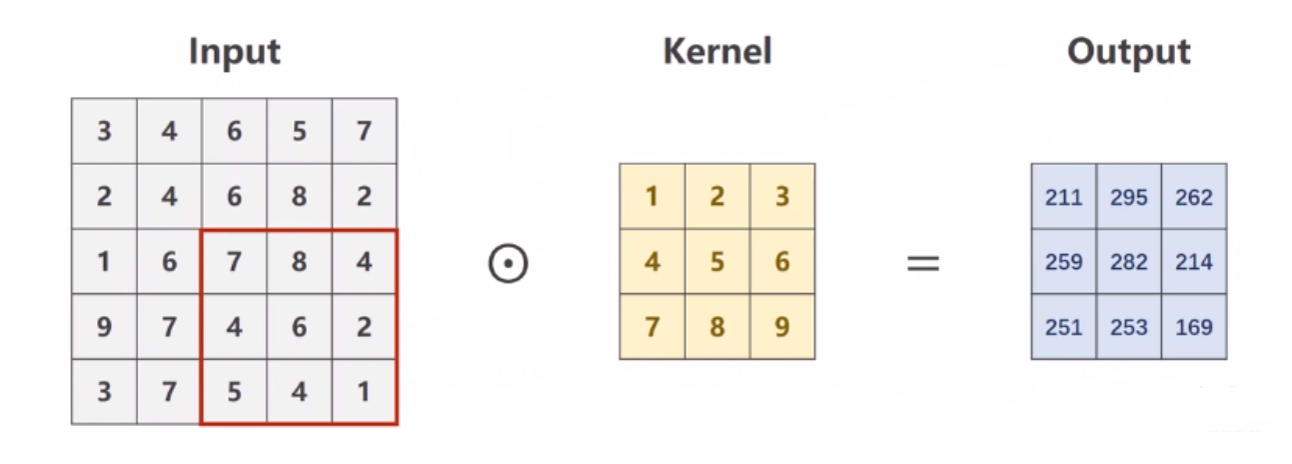
\includegraphics[width=14cm]{pic/conv-compute.png}
	\caption{卷积核计算示意图}
	\label{conv-compute}
\end{figure}

在图\ref{conv-compute}中,输入的是一个$5\times5$的特征图,卷积核大小为$3\times3$,步长为1,不做填充,则输出是一个$3\times3$的特征图。
若做零填充,则可以输出一个与原特征图维度大小相同的$5\times5$的特征图,输出特征图的宽度$w_o = \frac{w_i-f+2p}{s}+1$,其中$w_o$和$w_i$分别表示输出、输入特征图宽度,$f$表示卷积核大小,$p$表示边缘零填充个数,$s$表示卷积核滑动步长。

\subsection{激活层}
卷积神经网络中的激活层是神经网络中重要的组成部分。它们为网络引入非线性,使得模型能够学习更加复杂的特征和模式,逼近更加复杂的函数,避免神经网络仅仅是线性变换的叠加。

\textbf{(1)Sigmod激活函数}

Sigmod激活函数的公式如下:
\begin{equation}
	\sigma(x) = \frac{1}{1+e^{-x}}
\end{equation}
该函数将输入变量压缩到$[0,1]$之间,常作为二分类问题的输出层,用于表示类别的概率。
其连续的平滑曲线可以较好地拟合非线性关系。
Sigmod函数的导数可以通过自身表达出来:$\sigma(x)=\sigma(x)(1-\sigma(x))$,这一性质在反向传播算法中非常有用,可以简化计算。
其函数图像如下图所示:

\begin{figure}[h]
	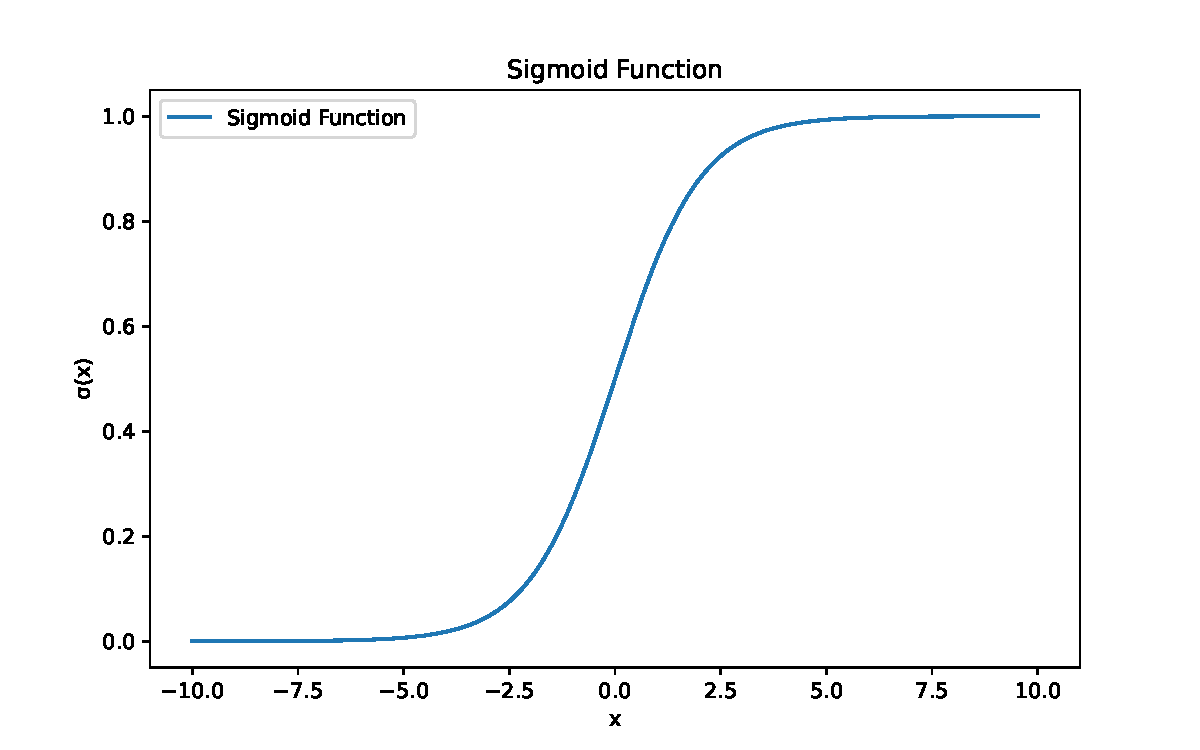
\includegraphics[width=8cm,height=5cm]{sigmod.pdf}
	\caption{Sigmod函数图像}
	\label{sigmod}
\end{figure}

但是,sigmod函数存在两个缺点:一是梯度消失问题,在函数的极端值区域(接近0或1),导数非常小,导致梯度在反向传播时消失,难以更新参数。
具体表现为,当x取极大或极小时,$\sigma^{'}(x)$非常接近0:$\sigma(x)=\sigma(x)(1-\sigma(x))\approx0$。
二是该函数函数的输出是非零均值,这可能导致后续层的输入不是零均值,从而影响梯度下降的效率。

\textbf{(2)ReLU激活函数}

ReLU激活函数的公式如下:
\begin{equation}
	r(x)=max(0,x)
\end{equation}

该函数不仅引入了非线性,而且将负数输出为0,引入了稀疏性。因其简洁和有效的特性,在许多神经网络中成为默认激活函数。

其函数图像如下图所示:

\begin{figure}[h]
	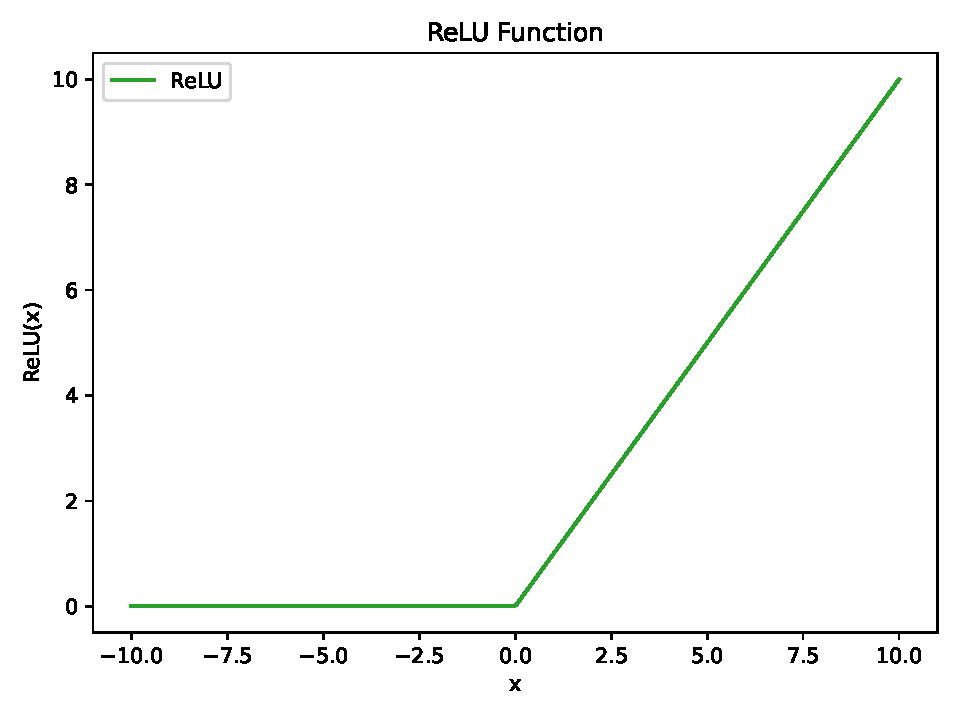
\includegraphics[width=8cm,height=5cm]{relu.pdf}
	\caption{ReLU函数图像}
	\label{relu}
\end{figure}

该函数不仅计算简单,而且不会将大部分输入映射到非常小的梯度,从而减轻了梯度消失问题,这有助于训练深层网络。
ReLU函数也能够加速随机梯度下降(SGD)的收敛速度,这是因为它的梯度在正半轴恒定为1,加速权重更新。

但是,ReLU 函数的一个缺点是“死亡 ReLU”现象,即一些神经元在训练过程中可能永久地输出零,这通常发生在学习率较大或偏置初始化不当时。解决方法包括使用小的正偏置初始化、降低学习率,或者使用变种ReLu函数,比如Leaky ReLU或Parametric ReLU(PReLU)等。
另一个缺点是在某些情况下,可能导致梯度爆炸问题,特别是在深层网络中。尽管这种情况较少,但仍需要注意。


\subsection{池化层}
随着卷积层数量的增加,特征图的特征通道数会逐渐增加,此时模型计算量会激增。
池化指的是在保留原特征图局部特征的前提下,降低特征图空间维度,减小分辨率,
从而增大卷积核感受野,大幅减少模型计算量,加速模型训练和收敛,避免模型过拟合。

池化层方法主要包括最大池化、平均池化等。
最大池化指的是在每个池化窗口取最大值。该算法有利于提取区域的显著特征,尤其是边缘、纹理等图像特征;对低频噪声起到一定抑制作用。但其容易忽视图像部分细节,造成部分信息损失。
平均池化方法是在每个池化窗口取均值。该算法有利于保留图像信息,增加图像的平滑性。但是对异常噪声比较敏感,而且容易模糊图像显著特征。

综上考虑,本文裂缝图像更关注边缘和纹理等显著特征,因此采用最大池化的方法。最大池化层计算示意图,如下图所示:

\begin{figure}
	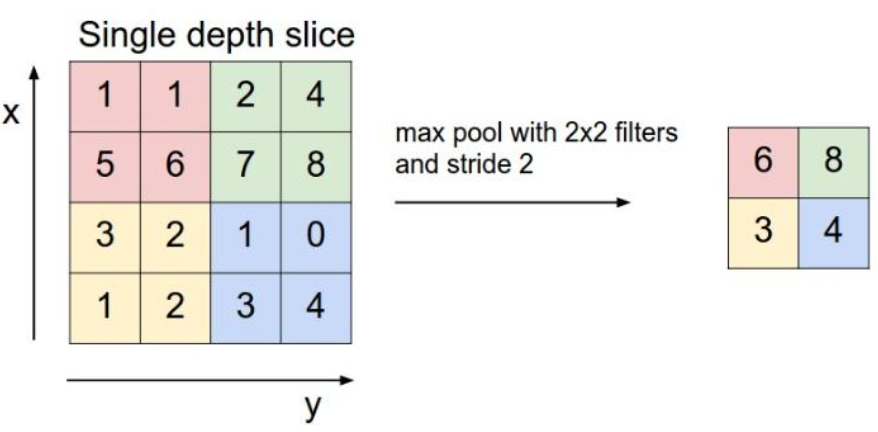
\includegraphics[width=14cm, height=7cm]{pic/pool-compute.png}
	\label{pool}
	\caption{最大池化层计算示意图}
\end{figure}

%————————————————————————————————————————————2.4 损失函数——————————————————————————————————————————————————————————————————————————
\section{损失函数}
损失函数(Loss Function)用于量化机器学习和统计模型中模型预测值与实际值之间的差异程度。
它在模型训练过程中起着至关重要的作用,指导模型优化算法(如梯度下降)调整模型参数以提高预测精度。
不同的任务和模型适用不同类型的损失函数。
本文裂缝检测模型的参数训练,采用交叉熵损失函数,下面对该损失函数做出详细介绍。

\subsection{softmax层}
Softmax层是神经网络中常用的一种输出层,该层将输入的未归一化的任意实数转换为归一化后的概率分布,确保输出的每个元素在0到1之间,并且所有输出的元素之和为1,常用于分类问题。

softmax函数公式如下:

\begin{equation}
	\mathbf{softmax}(z_{i})=\frac{e^{z_{i}}}{\sum_{j-1}^{K} e^{z_{j}}}
\end{equation}
上式中,$z_i$是向量$z$的第$i$的第i个向量。
本文U-Net模型最终的输出特征图包含两个特征通道,分别对应裂缝和背景。
该特征图经过softmax层输出每个通道上的概率分布,用于后续损失计算和像素类别预测。

\subsection{交叉熵损失函数}
交叉熵损失函数(Cross-Entropy Loss),主要用于衡量模型输出的概率分布与实际类别分布之间的差异,
该函数在深度学习和机器学习的分类任务中被广泛使用。

对于二分类问题,假设输出标签$y$为0或1,模型的输出$\hat{y}$是样本属于类别1的概率.
交叉熵损失函数定义为:

\begin{equation}
	\mathbf{Cross-Entropy Loss}=-\frac{1}{n}\sum_{i=1}^{n}[{y_i}log{\hat{y_i}} + (1-y_i)log(1-\hat{y_i})]
\end{equation}
其中。$y_i$是第$i$个样本的真实标签(0或1),$\hat{y_i}$是模型对第$i$个样本预测为1的概率,$n$为样本的数量。

本文裂缝图像的检测与识别,是在像素级别上进行裂缝和背景两个类别的分类,采用交叉熵作为参数训练的损失函数。


%————————————————————————————————————————————2.5 最优化方法——————————————————————————————————————————————————————————————————————————
\section{最优化方法}
在深度学习中,最优化方法指的是寻找损失函数最小化对应的模型参数的方法。
业界常用的最优化算法包括梯度下降法、RMSprop、Adam方法、牛顿法等。

本文裂缝图像检测,采用Adam优化器,该优化器结合了动量梯度下降和RMSprop的优点,通过对一阶和二阶矩的估计来动态调整每个参数的学习率,在需多深度学习任务中表现了优越的性能,能有效避免局部最优等问题。

%————————————————————————————————————————————2.7 本章小结——————————————————————————————————————————————————————————————————————————
\section{本章小结}
本章对后续工作相关的技术原理和基础理论做了详细介绍。
首先,介绍了将会在模型训练和实验阶段使用的数据预处理技术原理,尤其图像增广技术,用于对原有数据集的数量和多样性进行扩充。
紧接着,介绍了深度卷积神经网络,包括其提出的意义和关键层的原理,尤其是卷积网对图像数据的位移不变性和空间局部性两个特性的高效利用。
最后,介绍了用于模型参数训练的损失函数和最优化方法,包括用于本文模型训练的交叉熵损失函数和Adam优化方法。